\documentclass[14pt, fleqn, xcolor={dvipsnames, table}]{beamer}
\usepackage[T2A]{fontenc}
\usepackage[utf8]{inputenc}
\usepackage[english,russian]{babel}
\usepackage{amssymb,amsfonts,amsmath,mathtext}
\usepackage{cite,enumerate,float,indentfirst}
\usepackage{cancel}
\usepackage{color}
\usepackage{hyperref}
\hypersetup{colorlinks,urlcolor=NavyBlue}

\usepackage{tikz}                   
\usetikzlibrary{shadows}

% \usepackage{enumitem}
% \setitemize{label=\usebeamerfont*{itemize item}%
%   \usebeamercolor[fg]{itemize item}
%   \usebeamertemplate{itemize item}}

\graphicspath{{images/}}

\usetheme{Madrid}
\usecolortheme{seahorse}
\renewcommand{\CancelColor}{\color{red}}

\setbeamercolor{footline}{fg=Blue!50}
\setbeamertemplate{footline}{
  \leavevmode%
  \hbox{%
  \begin{beamercolorbox}[wd=.333333\paperwidth,ht=2.25ex,dp=1ex,center]{}%
    Амосов Федор, СПбГУ
  \end{beamercolorbox}%
  \begin{beamercolorbox}[wd=.333333\paperwidth,ht=2.25ex,dp=1ex,center]{}%
    Санкт-Петербург, 2014
  \end{beamercolorbox}%
  \begin{beamercolorbox}[wd=.333333\paperwidth,ht=2.25ex,dp=1ex,right]{}%
  Стр. \insertframenumber{} из \inserttotalframenumber \hspace*{2ex}
  \end{beamercolorbox}}%
  \vskip0pt%
}
\newcommand\indentdisplays[1]{%
     \everydisplay{\addtolength\displayindent{#1}%
     \addtolength\displaywidth{-#1}}}
\newcommand{\itemi}{\item[\checkmark]}

\title{Построение VoR-дерева с использованием технологии MapReduce\\\small{}}
\author[]{
    \small{
        Амосов Федор, СПбГУ\\
        ~\\
        Руководитель: Волохов Антон, Яндекс
    }
}
\date{}

\begin{document}

    \begin{frame}
        \maketitle
        \small
    \end{frame}

    \section{Постановка задачи}  
    
        \begin{frame}{Постановка задачи}
            Дано
            \begin{itemize}
                \item $10^9$ точек из $\mathbb{R}^5$
                \item Метрика
                \item Кластер из $10^3$ машин
            \end{itemize}  
            Задача
            \begin{itemize}
                \item Распараллеленно построить структуру для эффективных $1$-NN и $k$-NN запросов в данной метрике
            \end{itemize}         
        \end{frame}
        
    \section{Определения}
        
        \begin{frame}{VoR-дерево}
            Определение
            \begin{itemize}
                \item VoR-дерево = R-дерево + диаграмма Вороного
            \end{itemize}  
            В нашей задаче
            \begin{itemize}       
                \item Евклидова метрика --- ?
                \item $1$--NN запрос за $O(\log n)$
                \item $k$--NN запрос за $O(k + \log n)$
            \end{itemize}                
        \end{frame}
        
        \begin{frame}{R-дерево}
            \begin{center}
	            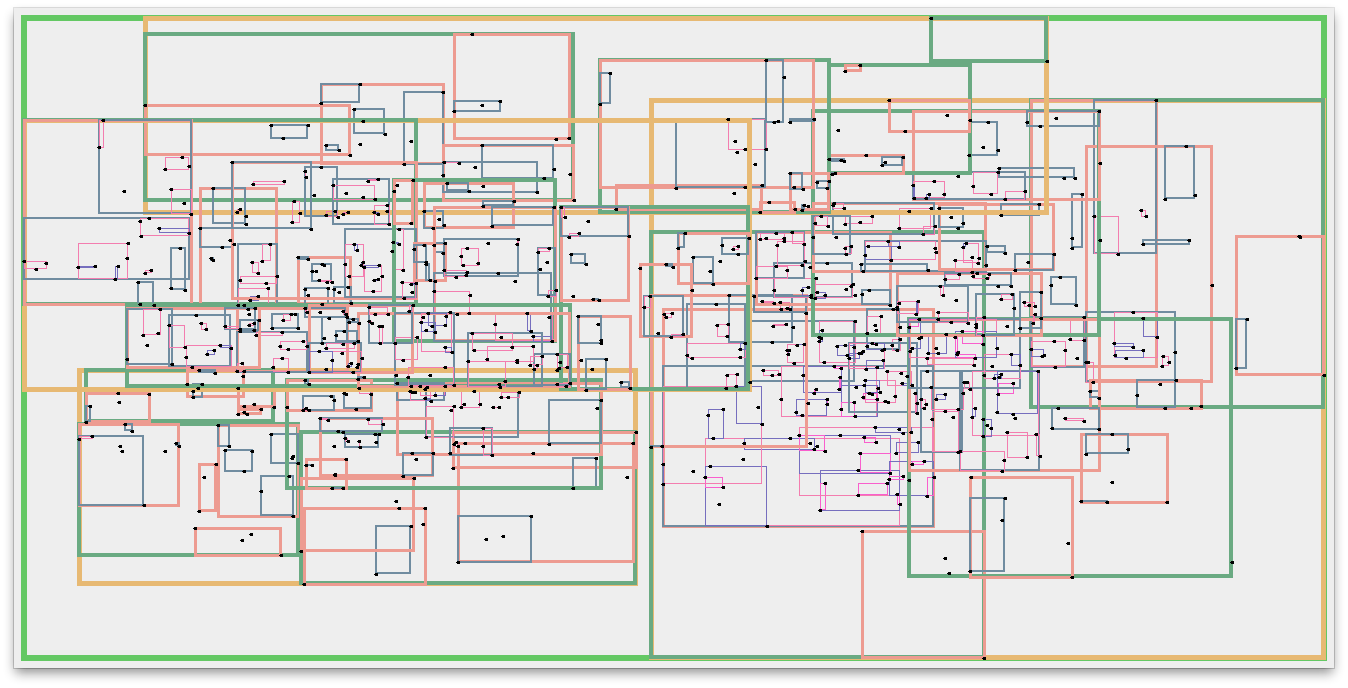
\includegraphics[scale = 0.25]{r-tree.png}
	        \end{center}  
        \end{frame}
        
        \begin{frame}{Диаграмма Вороного}
            \begin{center}
	            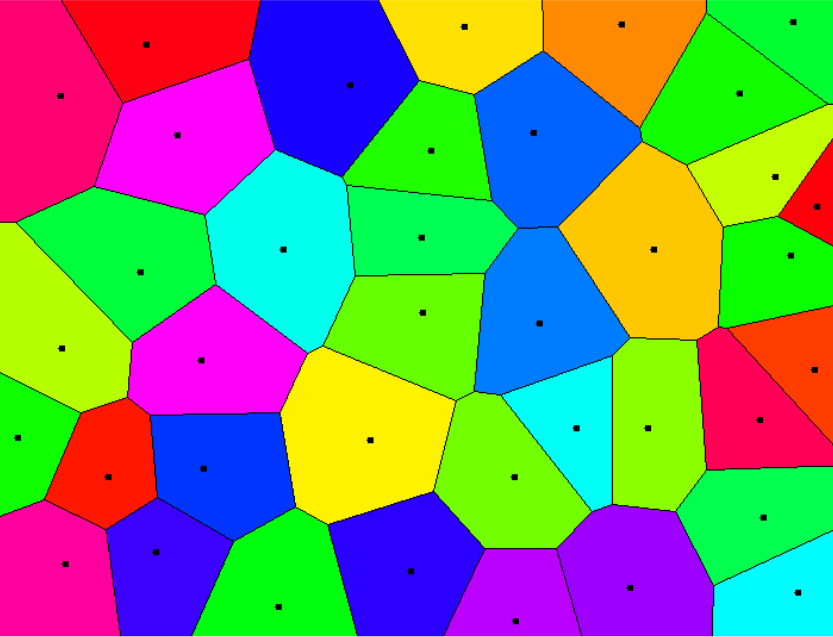
\includegraphics[scale = 0.33]{voronoi-1.png}
	        \end{center}       
        \end{frame}
        
        \begin{frame}{Диаграмма Вороного}
            \begin{center}
	            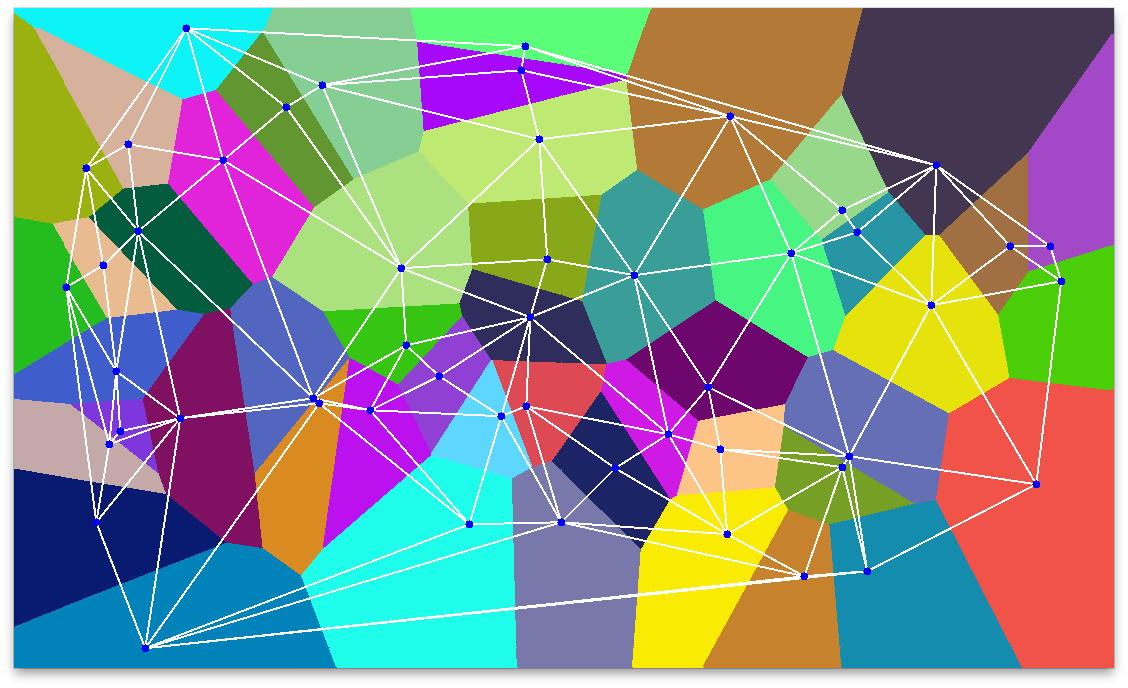
\includegraphics[scale = 0.33]{voronoi-2.png}
	        \end{center}       
        \end{frame}
        
        \begin{frame}{Граф Делоне}
            \begin{center}
	            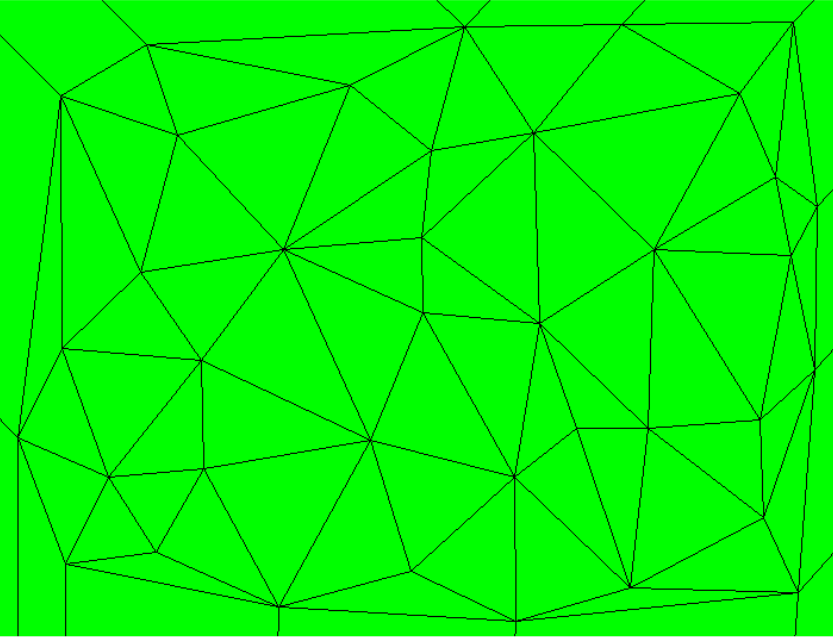
\includegraphics[scale = 0.33]{voronoi-3.png}
	        \end{center}       
        \end{frame}
        
        \begin{frame}{Основное свойство графа Делоне}
            \begin{center}
	            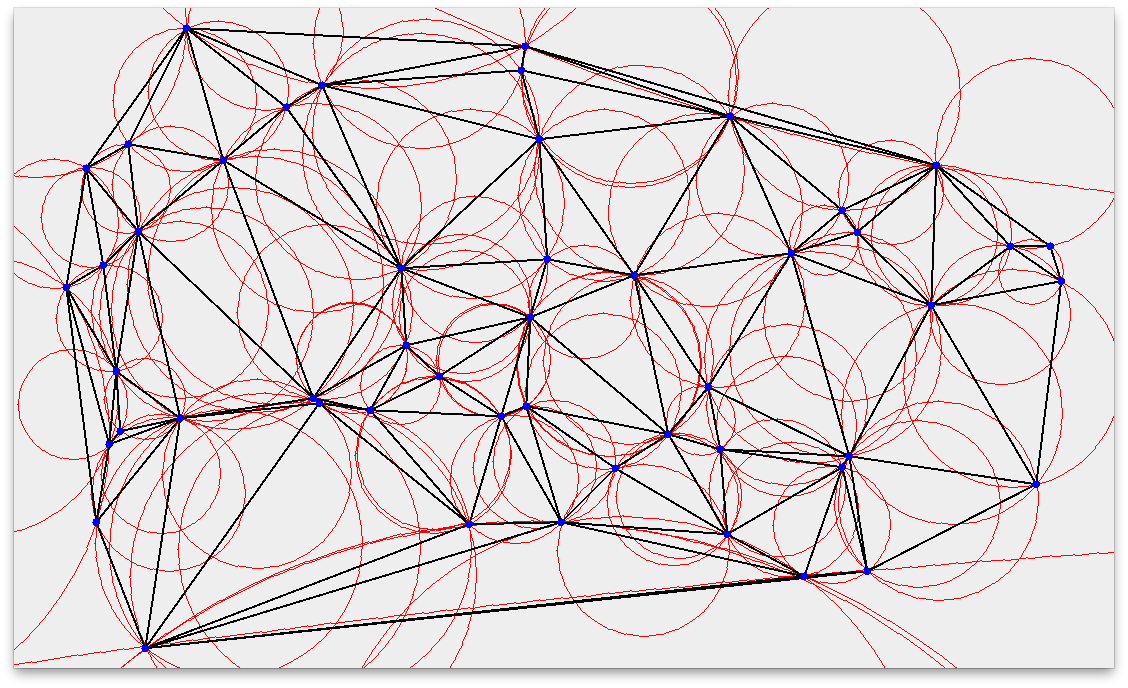
\includegraphics[scale = 0.33]{voronoi-4.png}
	        \end{center}       
        \end{frame}
        
        \begin{frame}{Плохие и хорошие треугольники}
            ~~~~~ Плохой треугольник ~~~~~~ Хороший треугольник
            \begin{center}
	            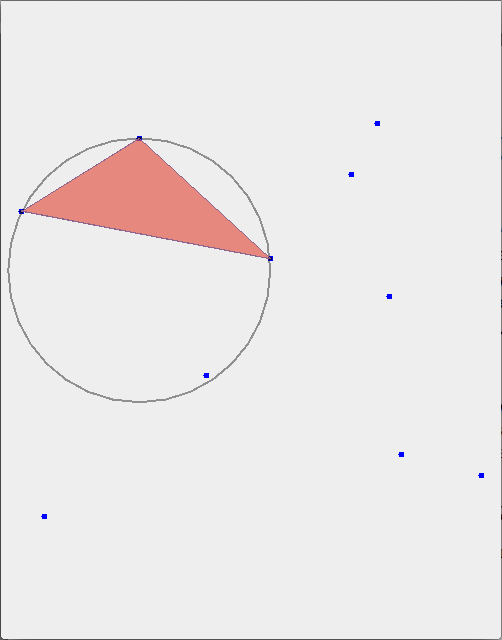
\includegraphics[scale=0.3]{creep.png}~~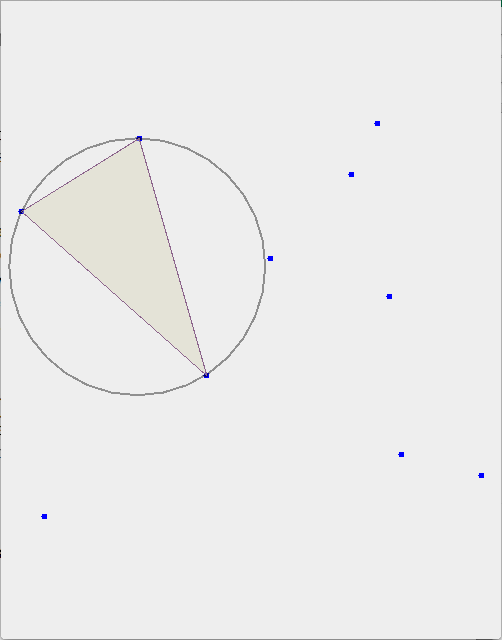
\includegraphics[scale=0.3]{no-creep.png}
	        \end{center}       
        \end{frame}
        
        \begin{frame}{VoR-дерево}
            \begin{center}
	            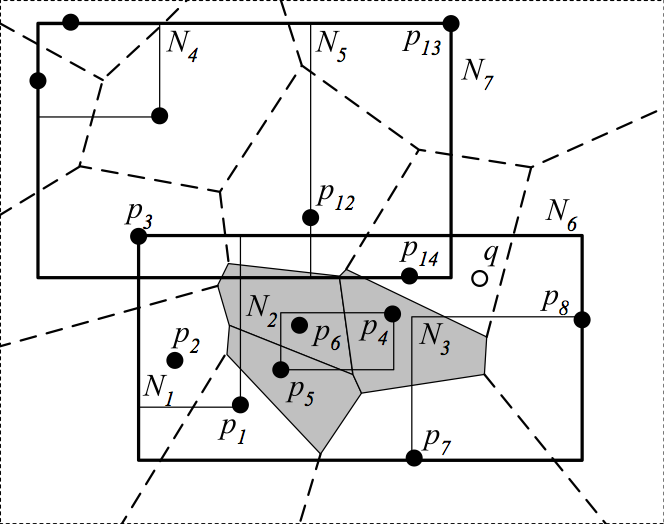
\includegraphics[scale = 0.3]{vor-tree.png}
	            
	            {\tiny Sharifzadeh , M., Shahabi C., <<VoR-Tree: R-trees with Voronoi Diagrams for Efficient Processing of Spatial Nearest Neighbor Queries>> Proceedings of the VLDB Endowment, 2010}	  
	        \end{center}   
        \end{frame}
        
    \section{Построение VoR-дерева}    
    
        \begin{frame}{Построение VoR-дерева}
            \begin{itemize}
                \item offline
                \item Требование распараллеленности $\Longrightarrow$ \\ <<разделяй и властвуй>> 
                \item Построить R-дерево за $O(n)$ --- очевидно
                \item Построить граф Делоне за $O(n \log n)$, следуя парадигме <<разделяй и властвуй>> --- ?
            \end{itemize}
        \end{frame}
        
        \begin{frame}{Построение графа Делоне 1}
            \begin{center}
                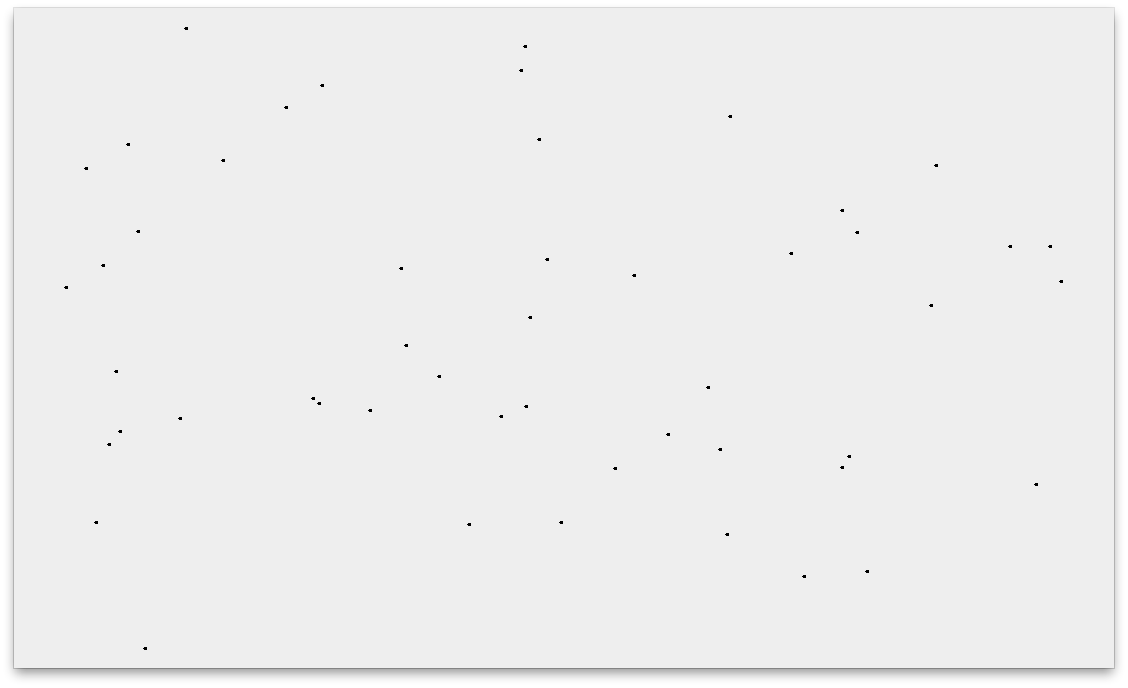
\includegraphics[scale=0.295]{1.png}
            \end{center}             
        \end{frame}
        
        \begin{frame}{Построение графа Делоне 2}
            \begin{center}
                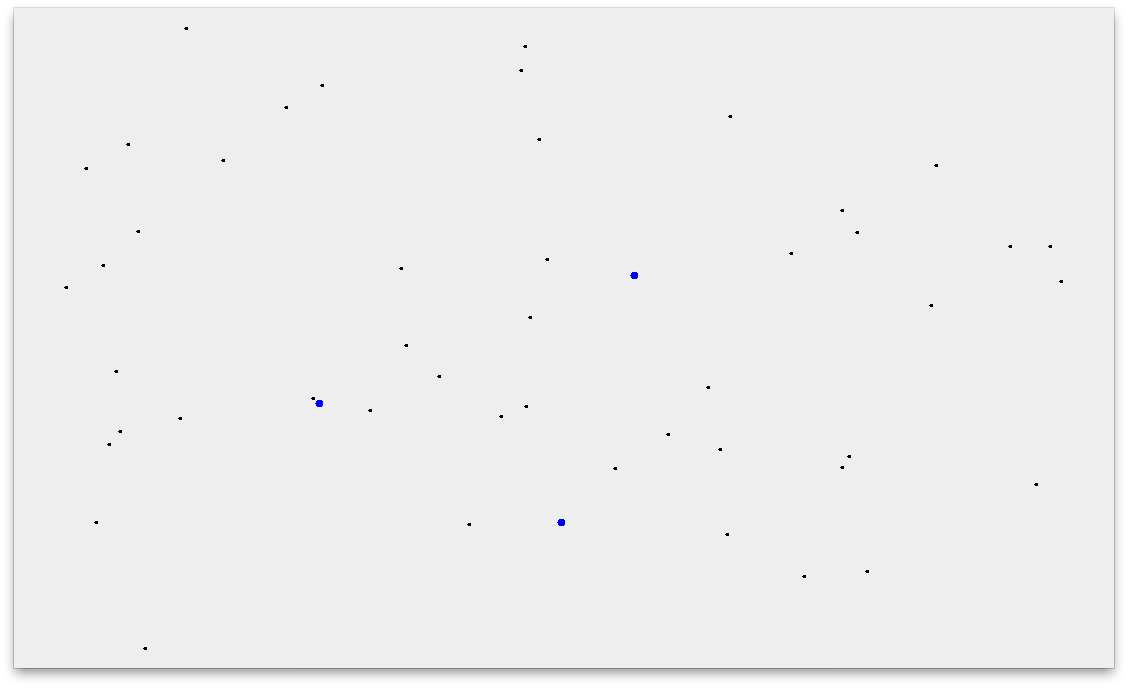
\includegraphics[scale=0.295]{2.png}
            \end{center}              
        \end{frame}
       

        \begin{frame}{Построение графа Делоне 3}
            \begin{center}
                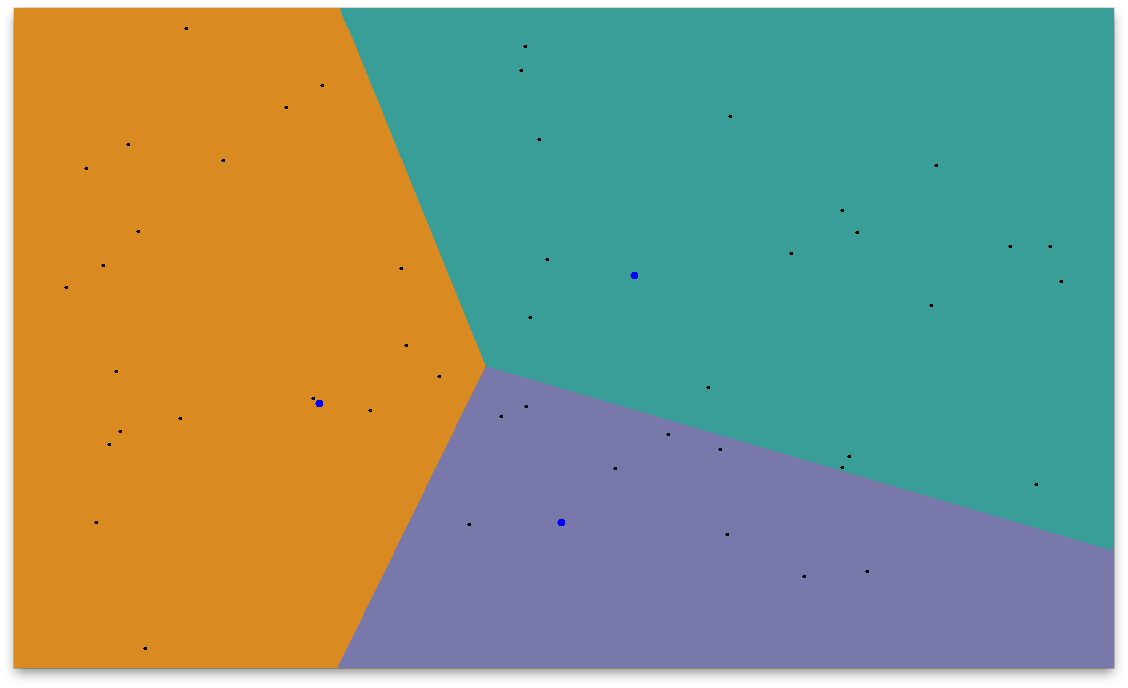
\includegraphics[scale=0.295]{3.png}
            \end{center}             
        \end{frame}
        
        \begin{frame}{Построение графа Делоне 4}
            \begin{center}
                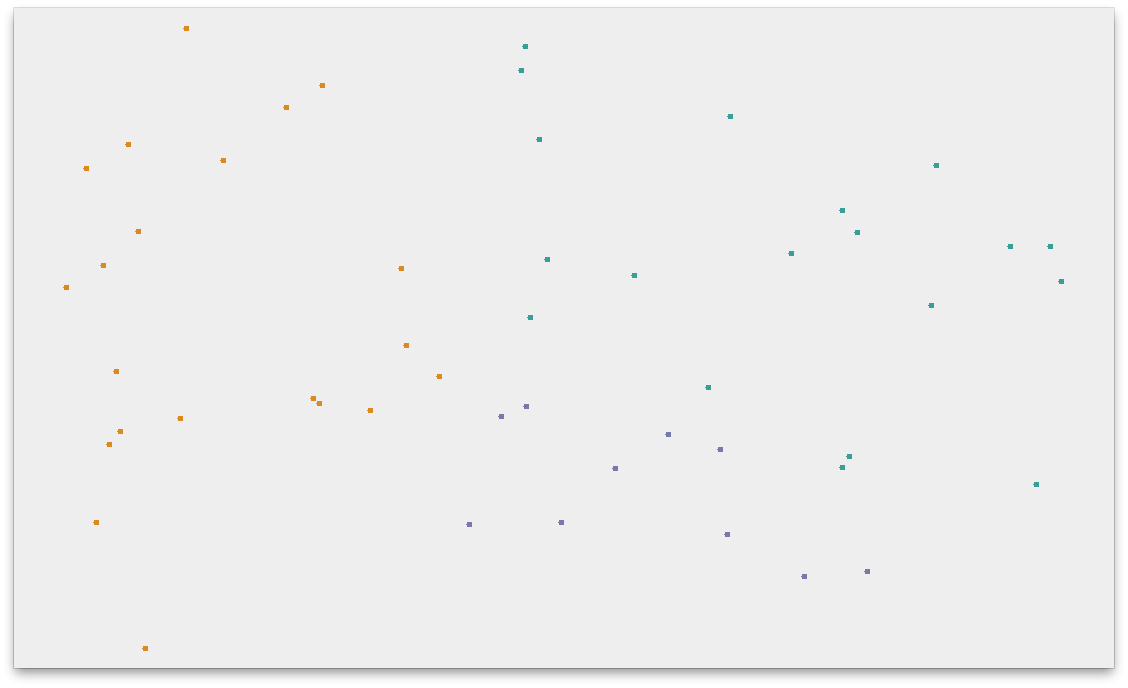
\includegraphics[scale=0.295]{4.png}
            \end{center}             
        \end{frame}
        
        \begin{frame}{Построение графа Делоне 5}
            \begin{center}
                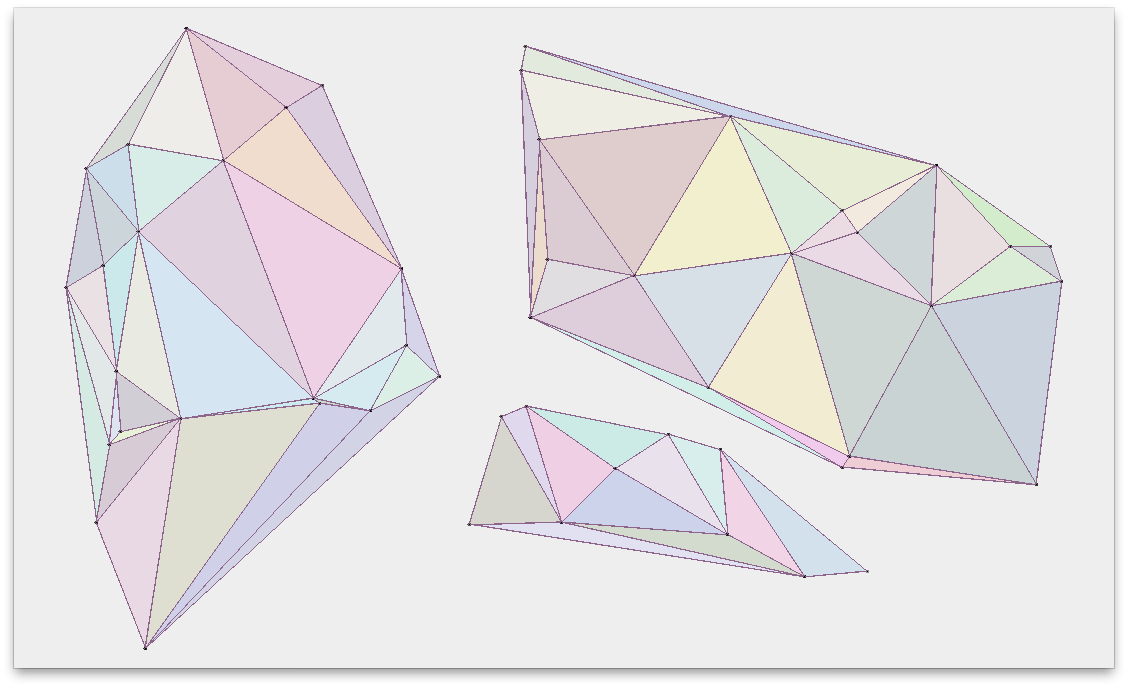
\includegraphics[scale=0.295]{5.png}
            \end{center}            
        \end{frame}
        
        \begin{frame}{Построение графа Делоне 6}
            \begin{center}
                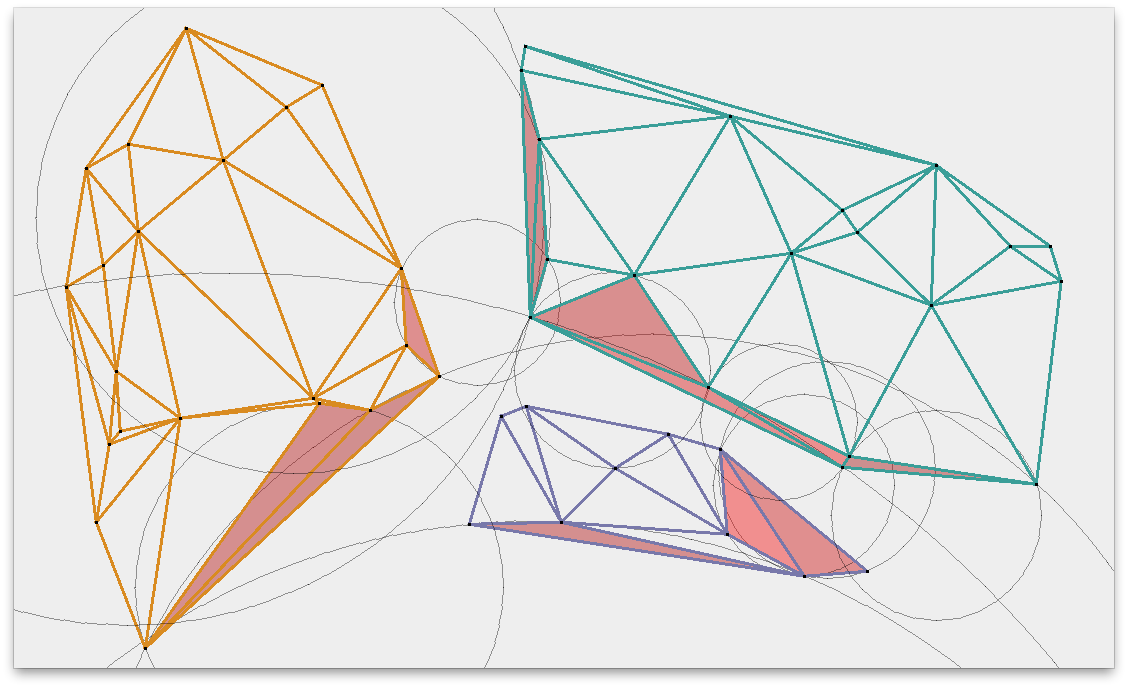
\includegraphics[scale=0.295]{6.png}
            \end{center}            
        \end{frame}
        
        \begin{frame}{Построение графа Делоне 7}
            \begin{center}
                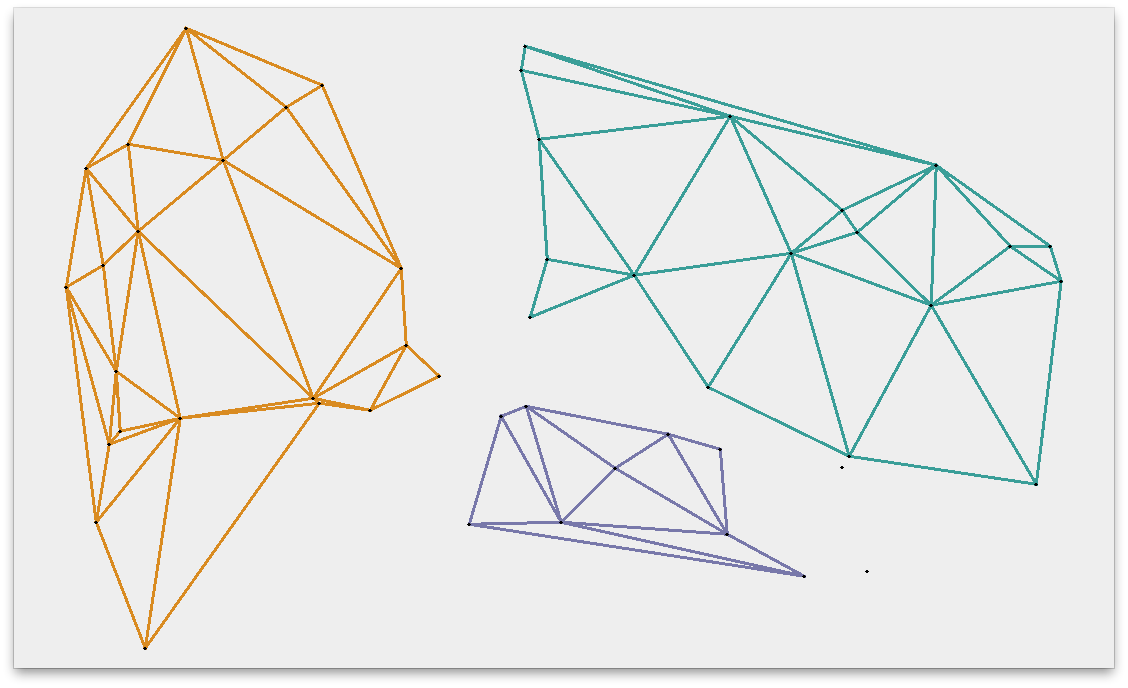
\includegraphics[scale=0.295]{7.png}
            \end{center}             
        \end{frame}
        
        \begin{frame}{Построение графа Делоне 8}
            \begin{center}
                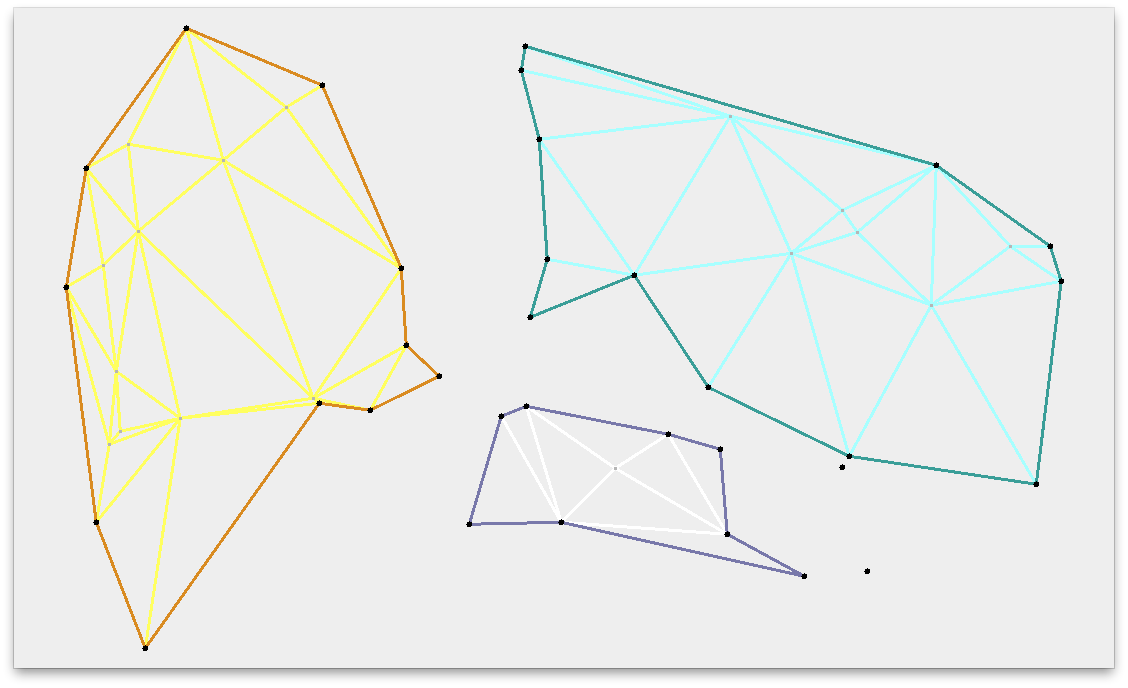
\includegraphics[scale=0.295]{8.png}
            \end{center}             
        \end{frame}
        
        \begin{frame}{Построение графа Делоне 9}
            \begin{center}
                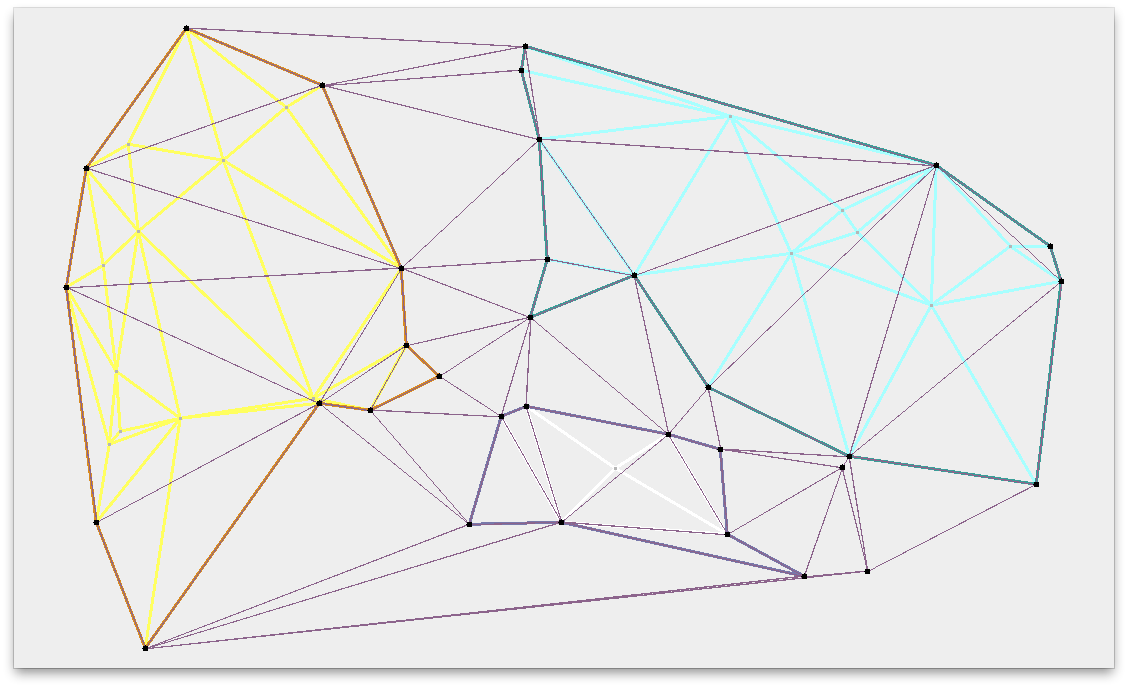
\includegraphics[scale=0.295]{9.png}
            \end{center}             
        \end{frame}    
        
        \begin{frame}{Построение графа Делоне 10}
            \begin{center}
                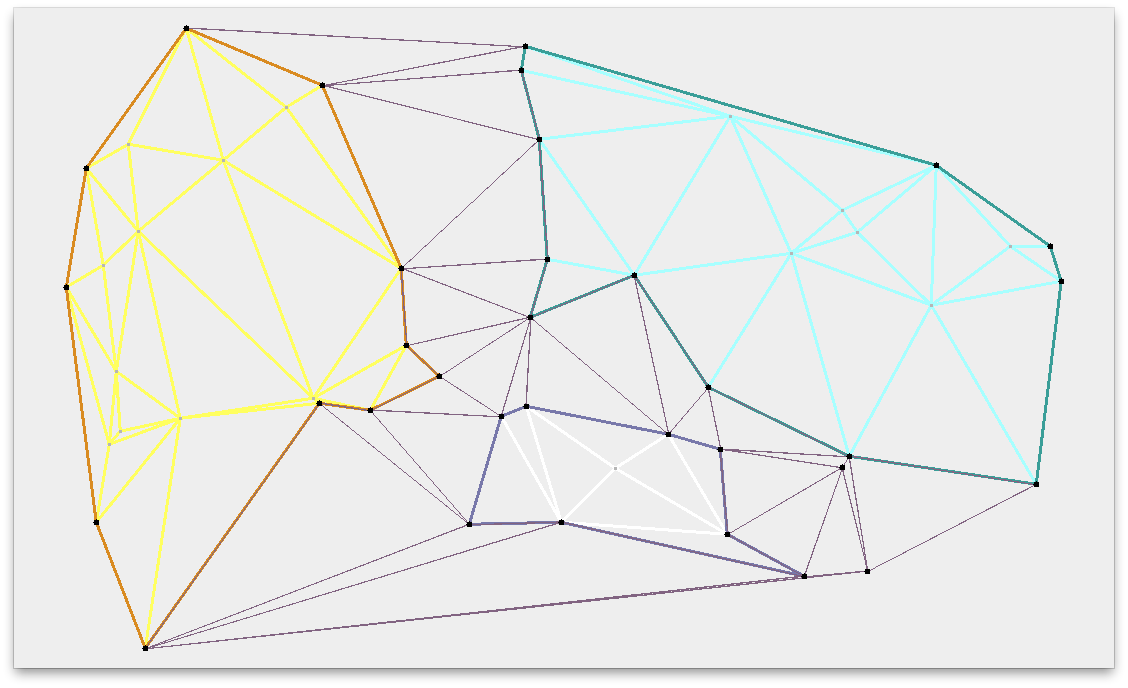
\includegraphics[scale=0.295]{10.png}
            \end{center}            
        \end{frame}  
       
        
        \begin{frame}{Построение графа Делоне 11}
            \begin{center}
                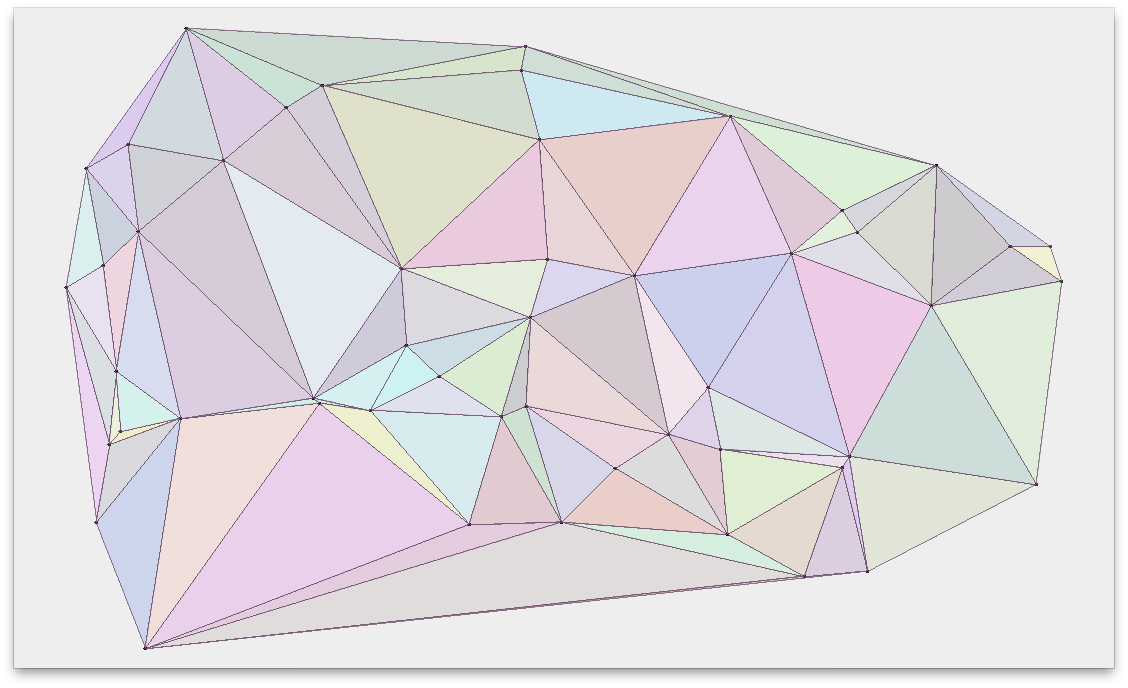
\includegraphics[scale=0.295]{11.png}
            \end{center}             
        \end{frame} 
        
        \begin{frame}{Наш алгоритм}
            \begin{enumerate}
                \item Разбить множество точек на несколько частей$^*$
                \item Построить на каждой части граф Делоне
                \item Удалить в каждом построенном графе <<плохие>> треугольники
                \item Добавить все оставшееся в итоговый граф 
                \item Построить на границах оставшегося <<склеивающий>> граф Делоне
                \item Добавить в итоговый граф ребра <<склеивающего>> графа
                    \begin{itemize}
                        \item соединяющие разные части
                        \item удаленные на 3 этапе
                    \end{itemize} 
            \end{enumerate}                       
        \end{frame}
        
    \section{Анализ алгоритма} 
        
        \begin{frame}{Анализ алгоритма}
            \begin{itemize}
                \item 2 утверждения $\Longrightarrow$ корректность
                \item Ускорение внешнего <<склеивающего>> алгоритма
                \begin{itemize}
                    \item $O(n^2) \longrightarrow O(n \log n)$
                    \item $O(n^k) \longrightarrow O(n^\frac{k}{2}), k > 2$
                \end{itemize}
            \end{itemize}
            
            %\begin{center}
            %    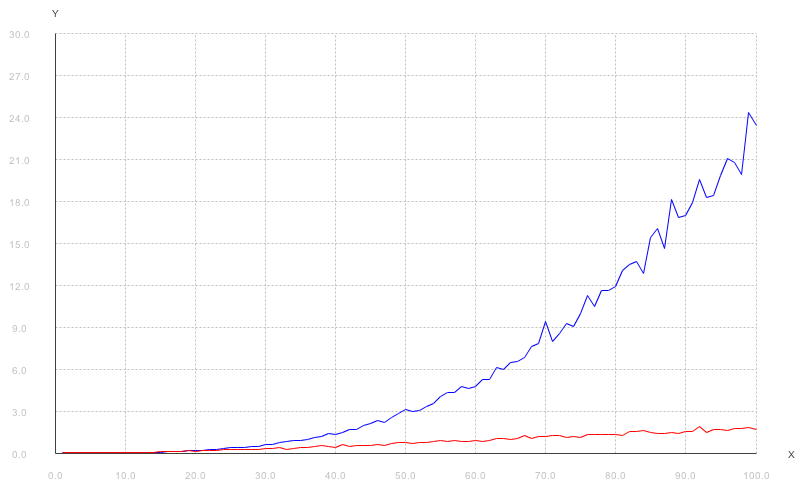
\includegraphics[scale=0.41]{comparison.png}
            %\end{center}           
        \end{frame}
        
        \begin{frame}{Улучшение алгоритма}
            \begin{enumerate}
                \item Плохие треугольники находятся вблизи границы $\Longrightarrow$ не надо проверять все треугольники
                \item Будем строить нашим алгоритмом сразу VoR-деревья  $\Longrightarrow$ определение <<хорошести>> треугольника с помощью построенных VoR-деревьев
                \item Склеивание можно проводить с помощью рекурсивного вызова нашего алгоритма. В чем подвох?
                \item Внешний алгоритм только для маленьких задач  
            \end{enumerate}
            Итого, сложность всегда $O(n \log n)$
        \end{frame}
        
        \begin{frame}{На практике}
            Ускорение наивного алгоритма
            \begin{center}
                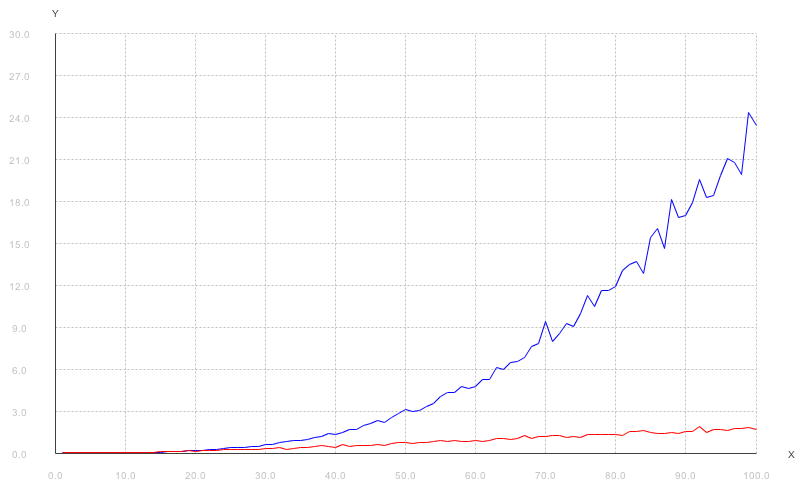
\includegraphics[scale=0.4]{comparison.png}\\
                Время работы от размера задачи   
            \end{center}  
                  
        \end{frame}
        
    \section{MapReduce}
        
        \begin{frame}{Распараллеливание 1}
            \begin{center}
                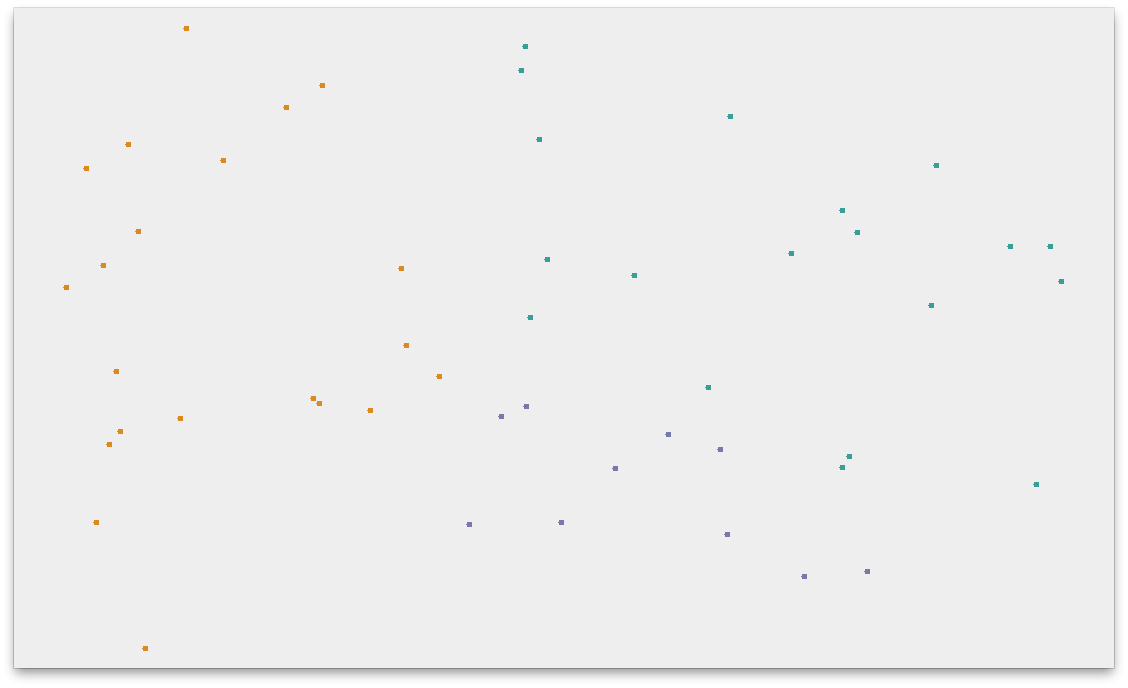
\includegraphics[scale=0.295]{4.png}
            \end{center}             
        \end{frame}
        
        \begin{frame}{Распараллеливание 2}
            \begin{center}
                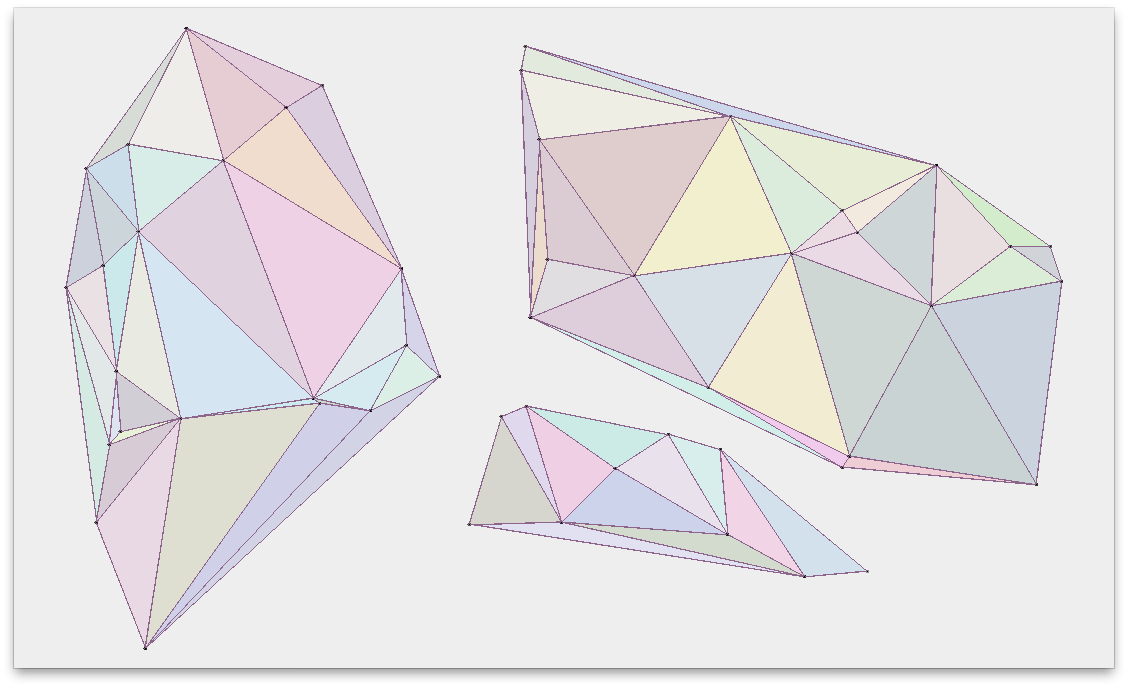
\includegraphics[scale=0.295]{5.png}
            \end{center}            
        \end{frame}
        
        \begin{frame}{Технология MapReduce}
            Технология
            \begin{itemize}
                \item Map --- обработка данных --- \\ построение VoR-деревьев из частей 
                \item Reduce --- свертка данных --- \\ склеивание полученных VoR-деревьев
            \end{itemize} 
            Реализация
            \begin{itemize}
                \item Apache Hadoop
                \item Сериализация VoR-дерева --- Google Protocol Buffers
            \end{itemize}              
        \end{frame}
        
    \section{Результаты}
    
        \begin{frame}{Результаты}
            Разработан алгоритм построения многомерного VoR-дерева
            \begin{itemize}
                \item Асимптотически эффективный 
                \item Хорошо параллелится
                \item Реализован на Java
                \item Реализован с использованием MapReduce
                \item Реализован с использованием MapReduce рекурсивно
            \end{itemize}
            До $10^9$ точек еще далеко, но прототип работает
        \end{frame}
        
        \begin{frame}{Q\&A}
            \begin{center}
                Спасибо за внимание!\\
                \href{https://github.com/amosov-f/VorTree}{github.com/amosov-f/VorTree}
                %{github.com/amosov-f/VorTree}
            \end{center}
        \end{frame}
        

\end{document}